\chapter{Stereo video watermarking}
\markright{Stereo video watermarking}
\label{wat}
\phantomsection
%\addcontentsline{toc}{chapter}{Stereoscopic Video}

\section{Watermaking}

Digital watermarking consists in imperceptiby and persistently associating some extra information with some original content. \\
The basic watermarking workflow is presented in Figure XX.\\
\begin{figure}[h!]
\centering
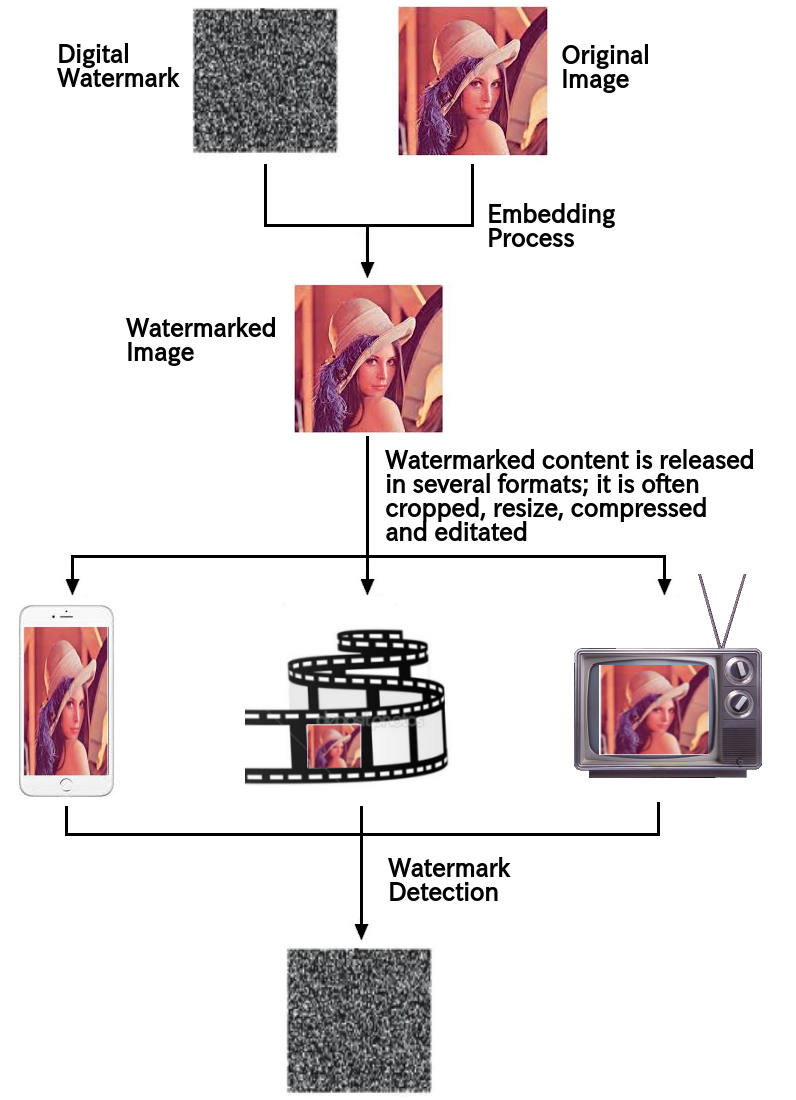
\includegraphics[width=0.3\textwidth]{./img/wat_workflow.png}
\caption{\small{Watermarking workflow}}
\label{fig:workflow}
\end{figure}
\newpage
\subsection{Properties}
Three parameters are required to evaluate watermarking technique performances:
\begin{itemize}
\item[-] transparency, that is the misure of how much the watermark affects the quality of the host data;
\item[-] robustness, i.e.,the capability of the hidden data to survive host signal manipulation including compression, signal processing, geometric manipulations;
\item[-] data payload, that is the amount of data of information bits that it is able to convey.
\end{itemize}
\begin{figure}[h!]
\centering
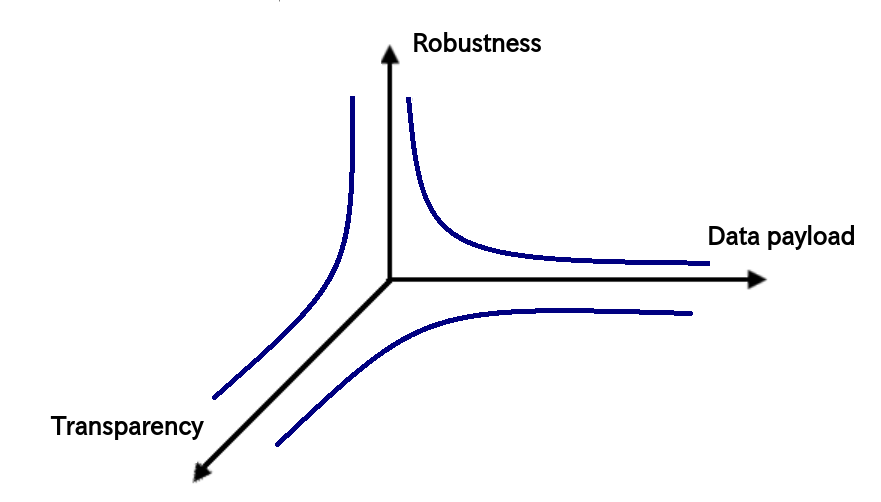
\includegraphics[width=0.4\textwidth]{./img/properties.png}
\caption{\small{Watermark properties trade-off}}
\label{fig:properties}
\end{figure}


Trasparenza articolo
\newline
Since in stereoscopic video context it is rather common practice to generate intermediate virtual views to adjust depth perception and since such view synthesis introduces non-rigid local geometric distortion that are not properly tackled by state-of-the art resynchronization mechanisms, stereo video watermarking strategies have to achieve robustness to synthetic view synthesis.


\subsection{Embedding techniques}
The most straightforward ways to add a watermark in a given content have been proved to be Spread Spectrum (SS) approach and Side Information (SI).\\
\begin{figure}[h!]
\centering
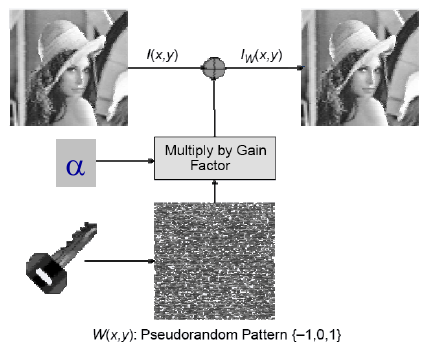
\includegraphics[width=0.4\textwidth]{./img/ss.png}
\caption{\small{Spread spectrum technique}}
\label{fig:ss}
\end{figure}
As in spread spectrum communications, the former approach considers the original
content as a signal and the watermark as a noise that is spread over very many frequency bins so that the energy in any one bin is very small and certainly undetectable.\\
The latter takes advantage of the fact that the original content is known at the
embedder side (but unknown at the detector): this way the watermark can be modulated  according to the original and the quantity of
inserted data can be maximed.\\

\subsection{Embedding domains}
Host features modified during embedding can
belong to 
\begin{itemize}
\item[-] spatial domain: the watermark is embedded by directly modifying the pixel values;
\begin{figure}[h!]
\centering
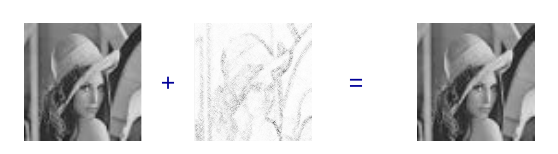
\includegraphics[width=0.4\textwidth]{./img/domain1.png}
\caption{\small{Spatial domain watermark insertion}}
\label{fig:dom1}
\end{figure}
\item[-] frequency domain: the image is transformed through a mathematical transformation, some coefficients are modified and finally the inverse transform is carried out;
\begin{figure}[h!]
\centering
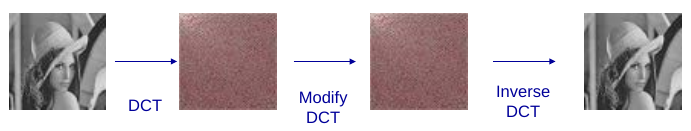
\includegraphics[width=0.4\textwidth]{./img/domain2.png}
\caption{\small{Frequency domain watermark insertion}}
\label{fig:dom2}
\end{figure}
\item[-] hybrid techniques: a block wise transform is applied, the image is divided
into blocks and for each block a mathematical transformation is computed, some coefficients are modified and the inverse transform is done.
\begin{figure}[h!]
\centering
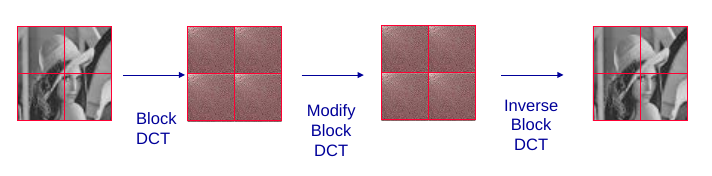
\includegraphics[width=0.4\textwidth]{./img/domain3.png}
\caption{\small{Hybrid technique}}
\label{fig:dom3}
\end{figure}
\end{itemize}

In stereoscopic video context the studies can also be structured in two other categories:
\begin{itemize}
\item[-] view-based methods;
\item[-] disparity-based methods
\end{itemize}
according to the reference image in which the mark is actually inserted.\\
In Figures XX and XX the workflows of both methods are presented.
\begin{figure}[h!]
\centering
\begin{subfigure}[]{0.4\textwidth}
\centering
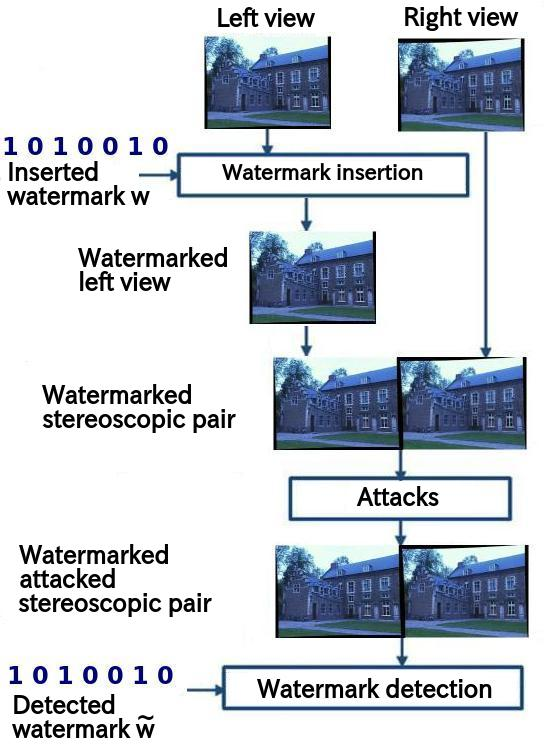
\includegraphics[width=0.8\textwidth]{./img/views_domain.jpeg}
\caption{\small{View-based watermarking workflow}}
\label{fig:view}
\end{subfigure}% 
~ %add desired spacing between images, e. g. ~, \quad, \qquad,  etc.$  $
  %(or a blank line to force the subfigure onto a new line)
\begin{subfigure}[]{0.4\textwidth}
\centering
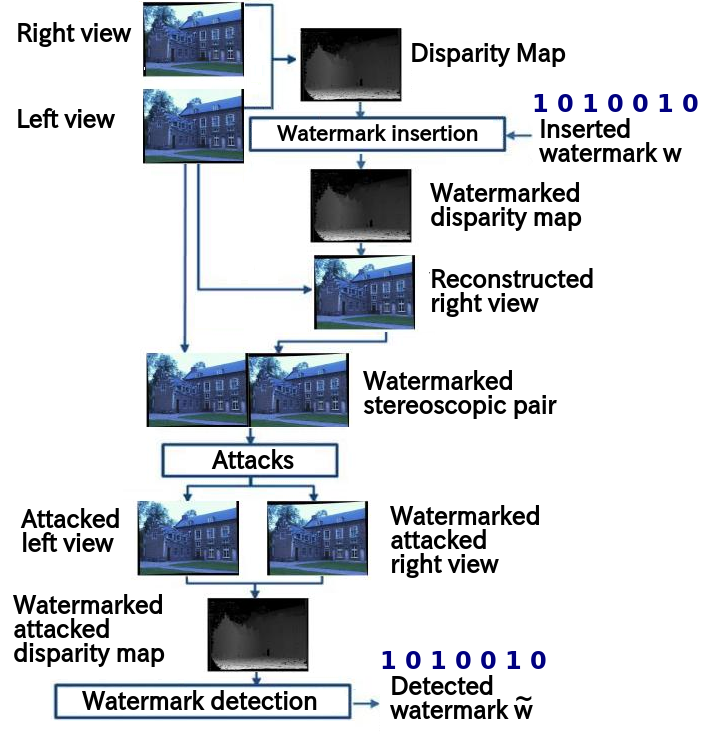
\includegraphics[width=1.05\textwidth]{./img/disparity_domain.png}
\caption{\small{Disparity-based watermarking workflow}}
\label{fig:disp}
\end{subfigure}
\caption{\small{Stereoscopic video watermarking workflow}}
\end{figure}


\section{Stereoscopic video watermarking}

\subsection{State of the art}



\newpage
In this thesis ....
due algoritmi di marchiatura presentati; il primo spaziale ss con rumore gaussiano etc.. 
il secondo ss nella frequenza additivo moltiplicativo...


data payload è ...
la trasparenza è stata valutata con ...
la robustezza è stata provata per view synthesis e compressione



